\subsubsection{Cross-Site Scripting (Weiland)}
Oft auch XSS genannt. Bei einem Angriff mit Cross-Site-Scripting wird eine Website, welche auch eine ansonsten vertrauenswürdige Seite sein kann, vom Angreifer mit einem Script versehen, welches im Browser des Opfers ausgeführt wird. Dadurch kann auch die digitale Identität des Opfers gestohlen werden (siehe \gref{sec:content_security_session-hijacking} )\\ %Session-Hijacking
Dabei muss der Angreifer nicht zwangsläufig auf den Server zugreifen können. Dadurch, dass viele Seiten dynamisch gestaltet sind, bieten sich einem Angreifer viele Möglichkeiten. Zum Beispiel gibt es oft die Möglichkeit eine Kommentar zu hinterlassen. Wenn in solch einem Feld ein Script platziert wird, wird es vom Browser eines Betrachters automatisch ausgeführt.
\paragraph{Problem}
Es gibt grundsätzlich drei verschiedene Arten von Cross-Site-Scripting:
\subparagraph{reflektiert oder nicht-persistent}
Bei dieser Art des XSS wird das Script vom Benutzer \enquote{geliefert} und nicht auf dem Server gespeichert. Die ist zum Beispiel möglich, wenn wie bei \autoref{lst:content_XSS_Vulnerable_reflected} eine vom Benutzer getätigte Eingabe direkt ausgegeben wird. Dies kann ebenso über GET- oder POST-Methoden funktionieren. So kann ein Angreifer einem Opfer mit dem Link zu der Seite und einem angefügten Script als z.B GET-Parameter (z.B. \texttt{input=<script type="text/javascript"> alert ('Dies sollte nicht passieren!'}) dazu bringen ein Script auszuführen
\begin{lstlisting}[style=custom, language=PHP, caption={ reflektiertes Cross-Site-Scripting Anfällig},label={lst:content_XSS_Vulnerable_reflected}]
<html>
	<head>
	<title> Cross-Site-Scripting</title>
	</head>

	<body>
		<?php
		if(isset($_GET['input'])) echo $_GET['input'];
		else echo "keine Eingabe get&auml;tigt";			
		?>
	</body>
</html>
\end{lstlisting}
\subparagraph{persistent oder beständig}
Bei dieser Vorgehensweise wird das Script auf der Website gespeichert und somit bei jeder Anfrage ausgeliefert wird. \\ Dies lässt sich leicht anhand eines Forums beschreiben:\\\\
Der Angreifer hinterlässt eine Nachricht im Forum, in der ein Script eingebaut ist. Sobald nun ein Besucher des Forums diese Nachricht lesen will, führt der Browser das Script aus.
\subparagraph{DOM-basiert oder lokal}
Hierbei wird das bereits in der Seite vorhandene Script, z.B. Javascript, dazu verwendet, das eigene Script zu platzieren.\\
Dies kann zum Beispiel bei der Auswahl der Sprache geschehen. Beim folgenden Beispiel (\autoref{lst:content_XSS_Vulnerable_DOM}) wird die Standard-Sprache in der URL mitgegeben und mittels JavaScript ausgelesen.
\begin{lstlisting}[style=custom, language=PHP, caption={DOM-Cross-Site-Scripting Anfällig},label={lst:content_XSS_Vulnerable_DOM}]
<select><script>
document.write("<OPTION value=1>"+document.location.href.substring(document.location.href.indexOf("default=")+8)+"</OPTION>");
document.write("<OPTION value=2>English</OPTION>");
</script></select>
\end{lstlisting}

Diese Seite kann nun durch mitgeben des Parameters  \texttt{default=<script type="text/javascript"> alert ('Dies sollte nicht passieren!'} dazu gebracht werden, dieses Script in den Code einzufügen und ausführen zu lassen. Dabei bemerkt der Server gar nichts von diesem Angriff, da der Code clientseitig verändert wird. 

\paragraph{Methoden um Vorzubeugen}
Die effektivste Methode um XSS vorzubeugen, ist jegliche Benutzereingabe zu verhindern und nur eine rein statische Website zu verwenden. Da dies in der Praxis jedoch meist nicht möglich ist, müssen andere Methoden verwendet werden.\\\\ 
Um XSS auf seiner eigenen Site zu verhindern sollten alle Eingaben, welche ausgegeben werden zum Beispiel mit dem Befehl \enquote{htmlspecialchars}(PHP) behandelt oder auf irgendeine andere Art encodiert werden. Dadurch werden alle Sonderzeichen durch die dafür vorgesehenen Zeichen in der jeweiligen Sprache umgewandelt ( z.B. htmlspecialchars: aus < wird \&lt;), wodurch kein ausführbares Script mehr vorliegt.\\\\
Ebenso ist es möglich alle vom Benutzer tätigbaren Eingaben mit einer Whitelist zu versehen. Dies bedeutet, dass nur Eingaben eines bestimmten Formats zugelassen werden (z.B. 01.01.2014). Jedoch ist diese Methode meist aufgrund vieler verschiedener erlaubter Eingabeformate (z.B. Forum) nicht möglich.\\\\
Manche Browser verhindern die Verwendung von reflektierten XSS automatisch, so wird beispielsweise bei Internet Explorer 11 diese Meldung (\autoref{fig:content_security_xss_ie}) ausgegeben, wenn die Seite \autoref{lst:content_XSS_Vulnerable_reflected} mit einem Script als input aufgerufen wird.

\begin{figure}[H]
\centering
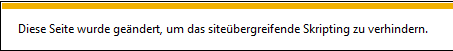
\includegraphics[keepaspectratio=true, width=10cm]{images/screenshots/xss_ie.png}
\caption{Internet Explorer blockiert reflektiertes XSS}
\label{fig:content_security_xss_ie}
\end{figure}

\paragraph{Samy}
Einer der bekanntesten Angriffe mittels XSS dürfte der Wurm \enquote{Samy} sein. Dieser wurde im Jahr 2005 erstellt und auf MySpace hochgeladen. Durch den Besuch der Seite von Samy's Entwickler wurde das Script ausgeführt, welches den Entwickler als Freund hinzufügte, den Text \enquote{but most of all, samy is my hero} auf die Pinnwand schrieb und das Script auf die eigene Seite schrieb, wodurch den Besuchers der eigenen Seite das selbe Schicksal blüht.
